\documentclass[conference]{IEEEtran}

\usepackage[spanish]{babel}
\usepackage{amsmath,amssymb,amsfonts,amsthm}
\usepackage{graphicx}
\usepackage[utf8]{inputenc} % Caracteres en Español (Acentos, ñs)
\usepackage{url} % ACENTOS
\usepackage{hyperref} % Referencias
\usepackage{float}

\usepackage{etoolbox}
\makeatletter
\patchcmd{\frontmatter@RRAP@format}{(}{}{}{}
\patchcmd{\frontmatter@RRAP@format}{)}{}{}{}
\makeatother	

\usepackage[backend=bibtex,sorting=none]{biblatex}
\addbibresource{references.bib}

\usepackage{datetime}
\newdateformat{specialdate}{\twodigit{\THEDAY}-\twodigit{\THEMONTH}-\THEYEAR}
\date{\specialdate\today}

\renewcommand\spanishtablename{Tabla}
\renewcommand\spanishfigurename{Figura}

\begin{document}

\title{Reporte Proyecto Individual U2 \\ Aplicación Móvil para Graficar Parabolas}

\author{\IEEEauthorblockN{Erika Daniela Mallozzi Martínez}
\IEEEauthorblockA{\IEEEauthorrefmark{} Ingeniería en Tecnologías de la Información\\
Universidad Politécnica de Victoria}
}

\maketitle

\begin{abstract} 
El presente informe describe el desarrollo de una aplicación móvil que permite graficar parabolas a partir de una ecuación de la forma \(y = ax^2 + bx + c\), donde \(a \neq 0\). La aplicación, desarrollada en Java para la plataforma Android, inicia con una parábola por defecto definida por la ecuación \(y = x^2\). Al realizar un gesto de doble clic sobre la gráfica, se abrirá una ventana emergente para editar la parábola e ingresar nuevos valores para \(a\), \(b\) y \(c\). Posteriormente, la aplicación regráfica la nueva parábola en función de los valores proporcionados por el usuario. La interfaz presenta una cuadrícula y un plano cartesiano para facilitar la visualización de la parábola graficada.
\end{abstract}

\section{Introducción}

La visualización y análisis de funciones matemáticas, como las parabolas, son herramientas fundamentales en la educación matemática y la investigación. El objetivo de este proyecto fue replicar la actividad de Geogebra titulada \textit{Demo: White border around the edge} \cite{parabola}  del autor Michael Borcherds, que permite a los usuarios interactuar con gráficas de parabolas. La aplicación desarrollada proporciona una interfaz intuitiva y amigable, permitiendo al usuario ingresar diferentes parámetros para graficar nuevas parabolas en tiempo real.

Esta aplicación móvil es de gran ayuda para entender como es que el cambio de los valores en las variables de la ecuación de una parábola, cambia de posición al tener la ecuación de una forma visual. 

\section{Desarrollo Experimental}

En este proyecto se desarrolló una aplicación móvil que utiliza el lenguaje de programación Java para la plataforma Android, replicando la funcionalidad de la actividad de Geogebra. Para llevar a cabo el desarrollo, se utilizó Android Studio como entorno de desarrollo integrado (IDE), aprovechando sus herramientas de diseño para implementar una interfaz gráfica intuitiva y funcional.

La aplicación comienza con una parábola predeterminada, \(y = x^2\). Al hacer doble clic en la gráfica, se activa un diálogo que permite al usuario ingresar nuevos valores para \(a\), \(b\) y \(c\) en la ecuación de la parábola \(y = ax^2 + bx + c\). Una vez que se ingresan los valores y se confirma, la aplicación regráfica la parábola utilizando los parámetros proporcionados. La interfaz incluye una cuadrícula y un plano cartesiano para facilitar la visualización.

\section{Resultados}

En esta sección se describen las principales características y funcionalidades de la aplicación de graficación de parabolas desarrollada. Se presenta la pantalla inicial de la aplicación, donde el usuario puede interactuar con la parábola predeterminada y acceder a la ventana emergente para modificar los parámetros de la ecuación.

Cuando el usuario ingresa nuevos valores y confirma la edición, la aplicación actualiza la gráfica para reflejar la nueva parábola. Además, se incluyen validaciones para garantizar que los valores ingresados sean correctos, mejorando así la experiencia del usuario.

A continuación se describe el funcionamiento detallado de las funciones de la aplicación:

En la Figura \ref{fig1}, se presenta la pantalla inicial de la aplicación, esto es lo que verá el usuario en primera instancia al abrir la aplicaxión móvil, es aquí donde el usuario puede navegar por el plano cartesiano con el gesto de desplazar el dedo de derecha a izquiera, así como arriba y abajo para visualizar la gráfica de la parábola base ( \(y = x^2\)).
\begin{figure}[H]
    \centering
    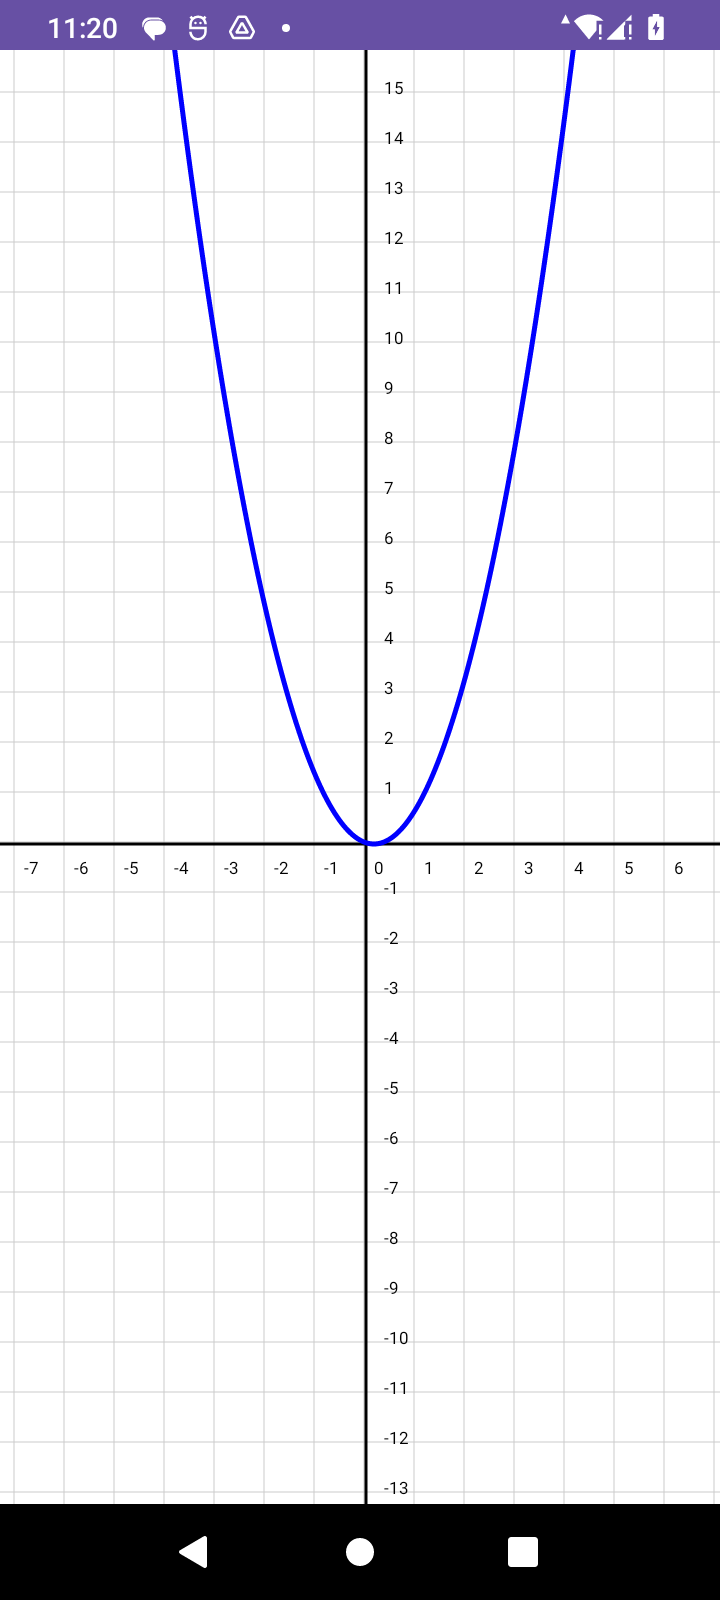
\includegraphics[width=0.4\columnwidth]{pantalla_inicial.png}
    \caption{Pantalla inicial de la aplicación graficación de parábola que muestra la parábola predeterminada.}
    \label{fig1}
\end{figure}



En la Figura \ref{fig2} se muestra el resultado de la acción del usuario al hacer el gesto de doble click en pantalla, se presenta una ventana de edición de la ecuación para graficación de la nueva parábola ingresada por el usuario.
\begin{figure}[H]
    \centering
    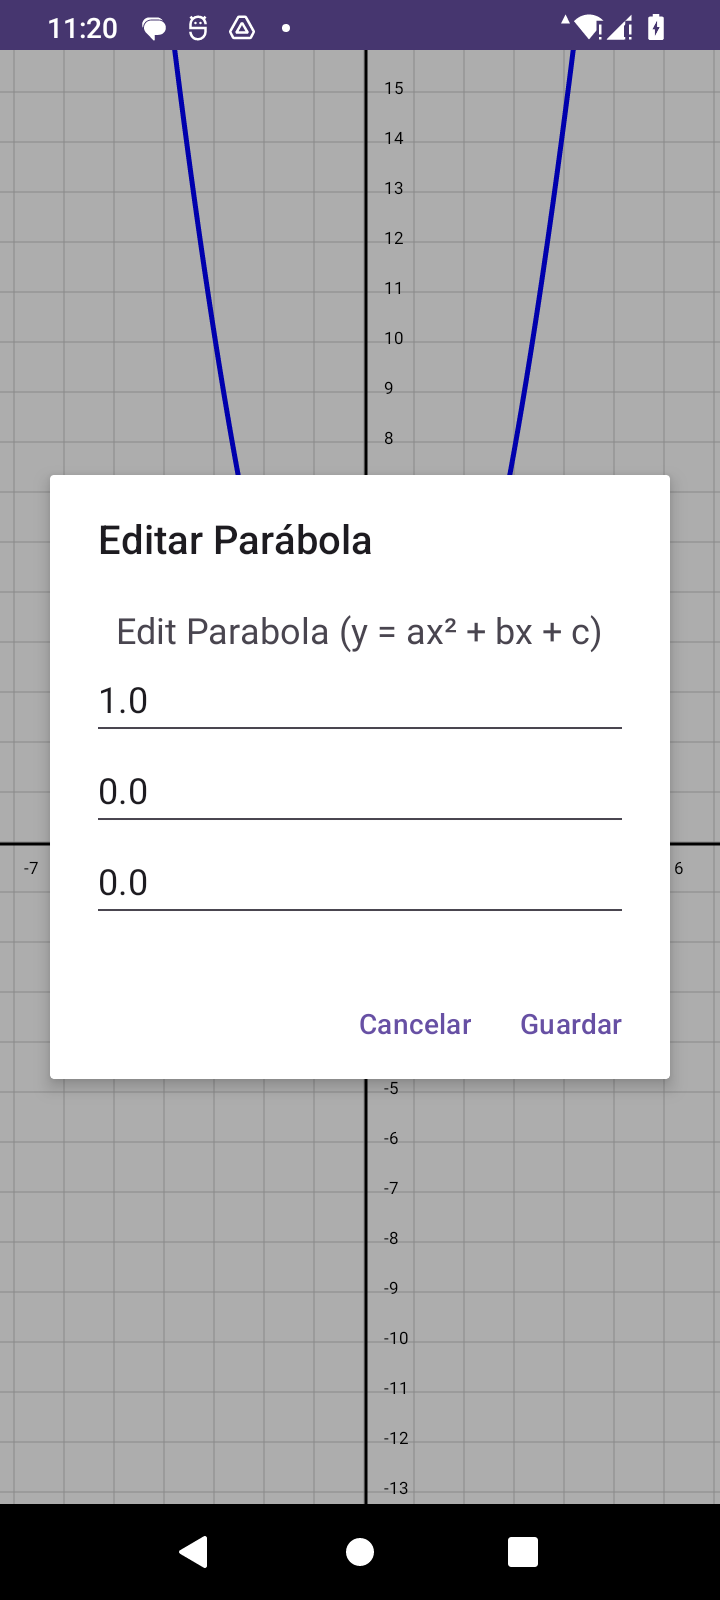
\includegraphics[width=0.4\columnwidth]{editar_parabola.png}
    \caption{Ventana emergente para la edición de variables en la ecuación.}
    \label{fig2}
\end{figure}



El usuario tiene la posibilidad de editar los valores de a, b y c en la ecuación, ingresar números negativos y flotantes, con la condición de que el valor de 'a' nunca puede ser igual a cero (0), y si es este el caso, se le presentará un mensaje en pantalla de 'El coeficiente a no puede ser cero'  \ref{fig3}.

\begin{figure}[H]
    \centering
    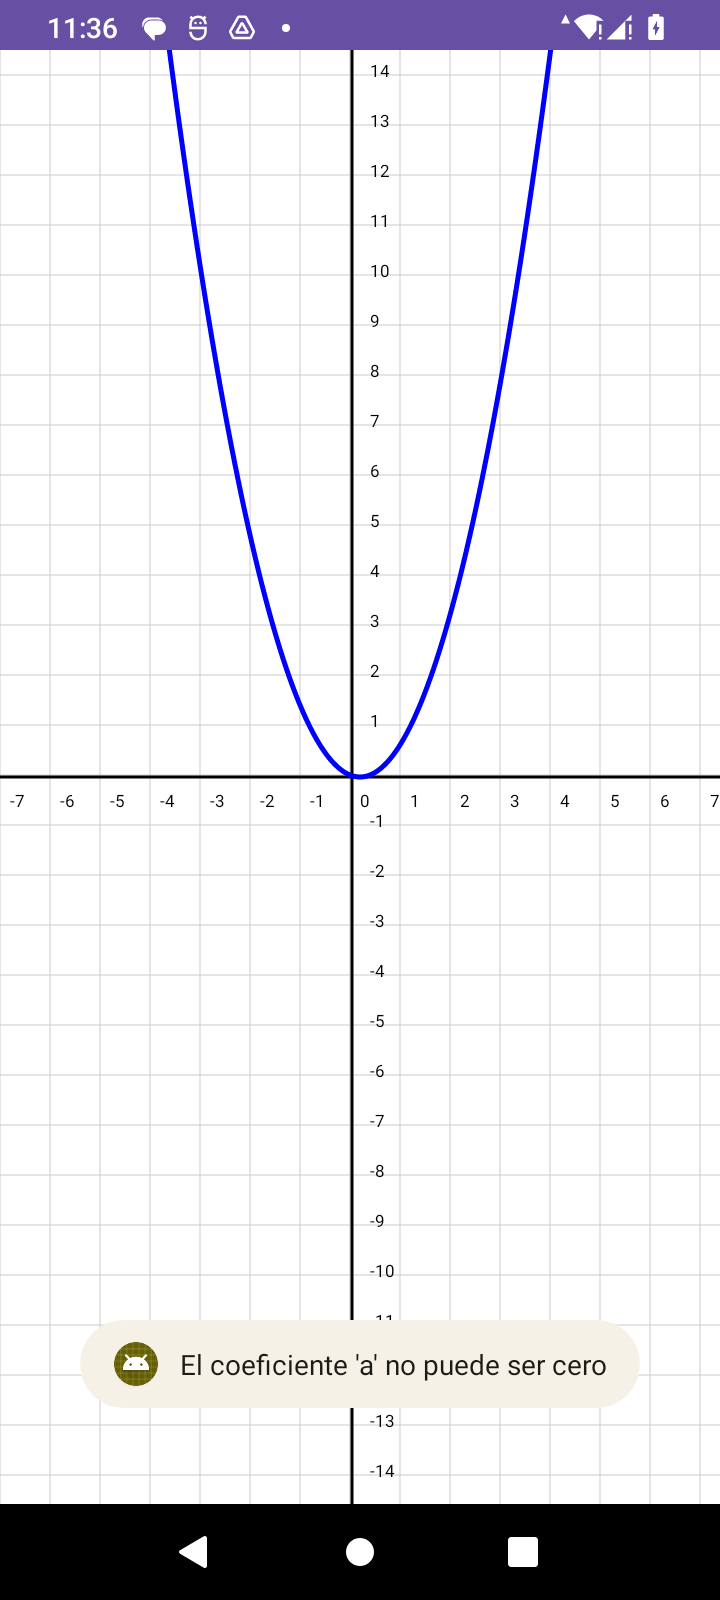
\includegraphics[width=0.4\columnwidth]{coeficiente_a_no_puede_ser_cero.png}
    \caption{Mensaje en pantalla sobre el coeficiente a no puede ser cero.}
    \label{fig3}
\end{figure}




Al terminar de editar los valores de las variables el usuario deberá clickear el botón de "Guardar", este botón se encuentra en la parte inferior derecha de la ventana emergente, ver esto en la Figura \ref{fig4}.
\begin{figure}[H]
    \centering
    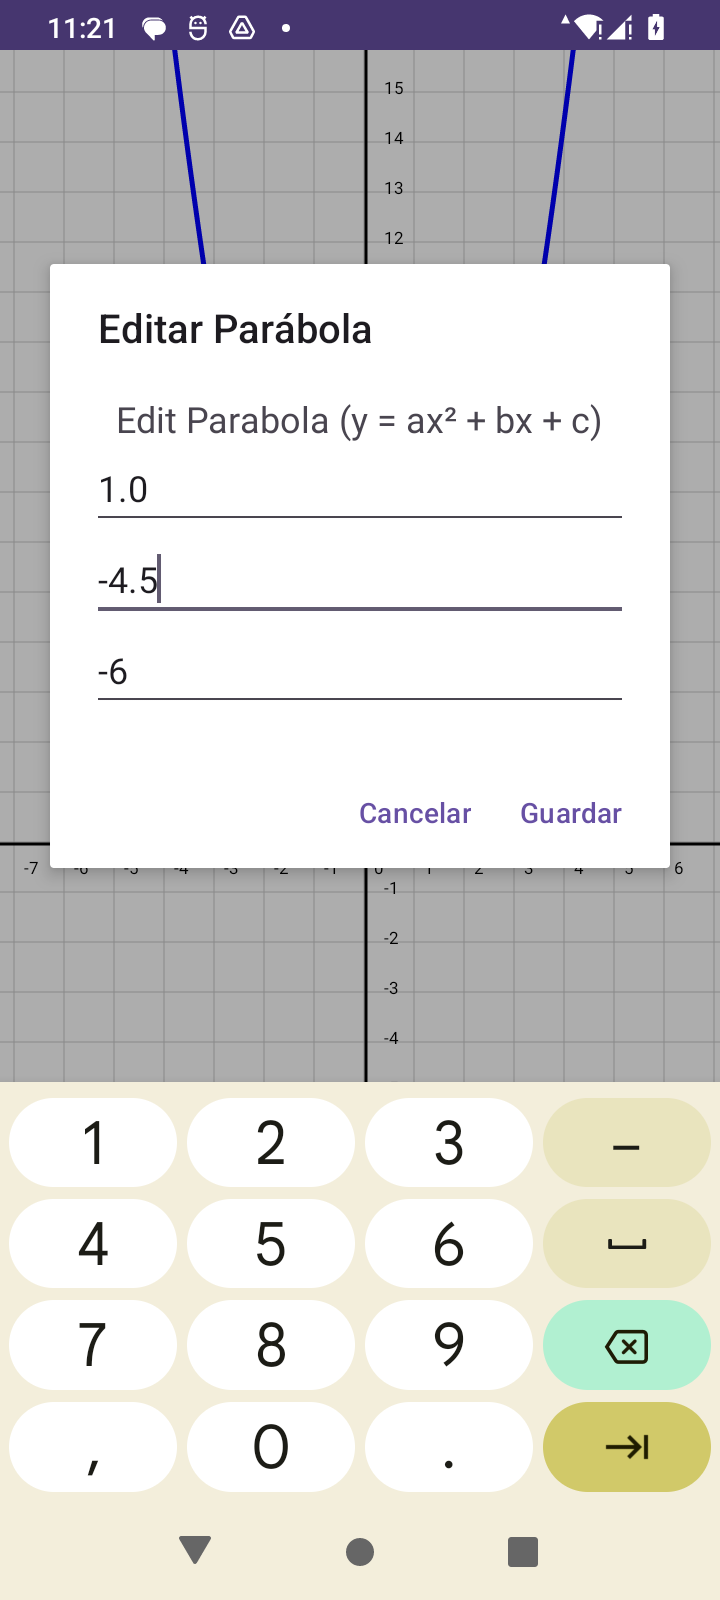
\includegraphics[width=0.4\columnwidth]{datos_nuevos.png}
    \caption{Valores de variables cambiados por el usuario.}
    \label{fig4}
\end{figure}






En seguimiento del proceso de graficación de la nueva parábola, después de que el usuario haya hecho click en el botón de "Guardar", se cerrará la pestaña de edición de parábola y se mostrará en el plano cartesiano la nueva parábola graficada correspondiente a la ecuación con los nuevos valores de las variables \ref{fig5},.
\begin{figure}[H]
    \centering
    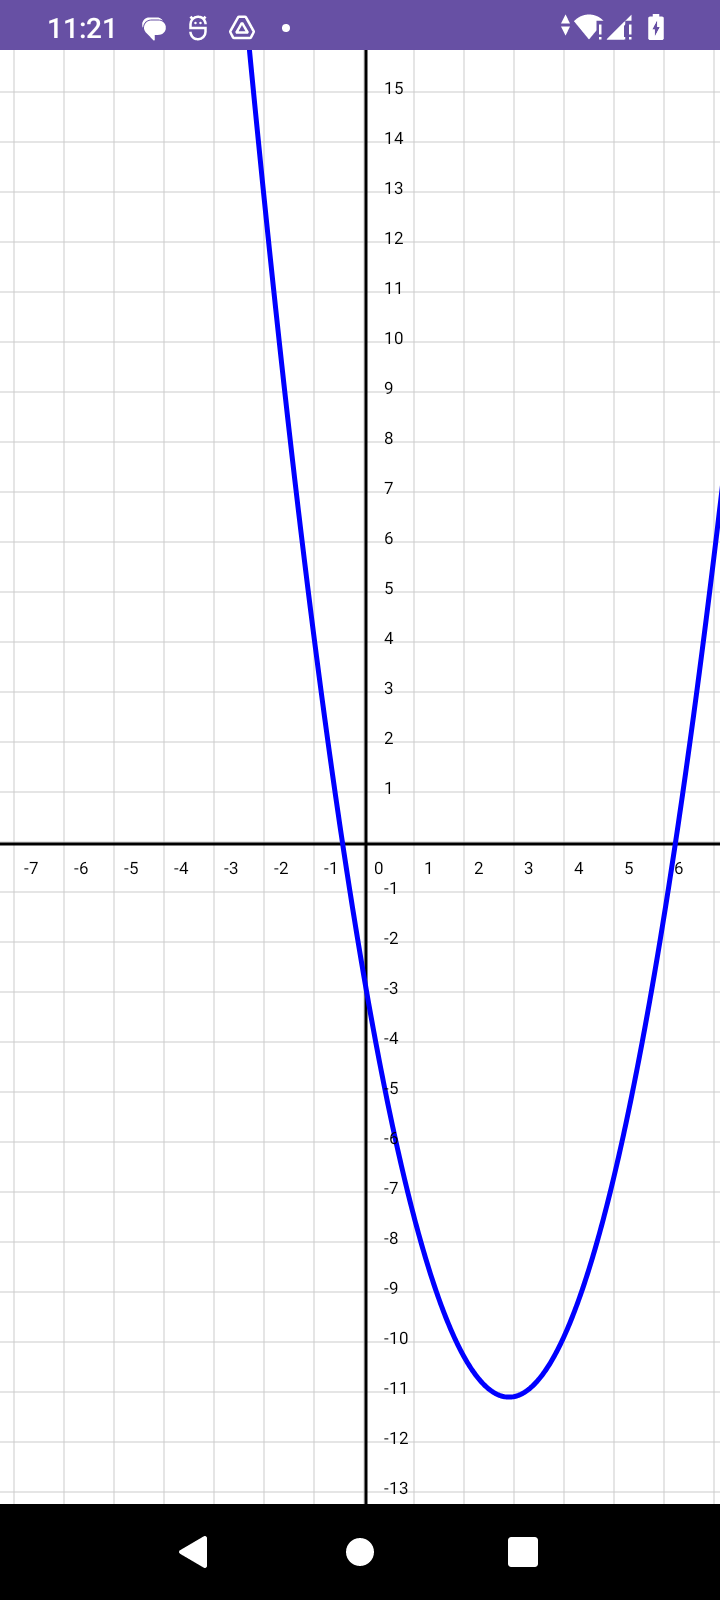
\includegraphics[width=0.4\columnwidth]{nueva_parabola.png}
    \caption{Cambio de gráfica de parábola por la nueva ecuación ingresada por el usuario.}
    \label{fig5}
\end{figure}



\section{Conclusión}

Este proyecto logró replicar la funcionalidad de la actividad de "Geogebra", proporcionando una herramienta útil para la visualización de parabolas en una aplicación móvil. La implementación de la aplicación en Java y el uso de Android Studio permitieron crear una interfaz intuitiva que facilita la interacción del usuario con las gráficas en el plano cartesiano.

Se lograron características clave como la edición dinámica de parámetros y la regráfica de la parábola en tiempo real, lo que enriquece la experiencia de aprendizaje y análisis matemático. Este desarrollo refuerza los conceptos fundamentales de programación en Android y la manipulación de gráficos, aplicando buenas prácticas de diseño de interfaces para dispositivos móviles.

\addcontentsline{toc}{section}{Referencias} 
\printbibliography

\end{document}
